\documentclass[french,nochapter,11pt]{rapportUB}  

\college{Collège Sciences et Technologies}
\uf{UF Mathématiques et Interactions}
\program{Master MAS parcours ROAD} %A remplir
\course{AONE} %A remplir
\academicyear{2024 -- 2025} %A remplir
\author{ %A remplir\\
	Matilin Periat
}

%Paquetages additionnels
\usepackage{placeins}
\usepackage{multirow}
\usepackage{framed}
\usepackage{amsmath}
\usepackage{algorithm2e}
\usepackage{tcolorbox}
\usepackage{stmaryrd}
\newcommand{\rb}{\rrbracket}
\newcommand{\lb}{\llbracket}
\usepackage{amsmath, amssymb, amsthm}
\usepackage{graphicx}
\usepackage{mathrsfs} % Pour \mathscr{P}
\usepackage{hyperref} % Pour des références cliquables

\newtheorem{proposition}{Proposition}

\usepackage[utf8]{inputenc}
%\usepackage[hidelinks]{hyperref}
%\usepackage[left=2cm,right=2cm,top=3cm,bottom=3cm]{geometry}
\usepackage{amsmath}
\usepackage{amsfonts}
\usepackage[T1]{fontenc}
\frenchbsetup{StandardLists=true}
\usepackage{enumitem}
\usepackage{array}
\usepackage{diagbox}
\usepackage{booktabs}
\usepackage{changepage} % Pour ajuster localement les marges
\usepackage{hyperref}
\usepackage{caption}
\usepackage{graphicx}
\usepackage{xcolor}
\usepackage{longtable}
\usepackage{makecell}



% Configuration de la couleur des liens hypertextes
% Voir https://www.overleaf.com/learn/latex/Hyperlinks
\hypersetup{
	colorlinks,
	linkcolor={red},
	citecolor={blue},
	urlcolor={blue}
}

%Pour gérer la bibliographie
\usepackage[backend=biber,style=numeric,giveninits=false,maxcitenames=10,minnames=1,maxnames=10,uniquename=full]{biblatex}

\addbibresource{Autre/biblio.bib}



\DeclareDelimFormat{nameyeardelim}{\addspace}  % Supprime la virgule entre les noms et l'année
\DeclareNameAlias{sortname}{given-family}      % Affiche "Prénom Nom" au lieu de "Nom, Prénom"

%Déclaration d'un nouvel opérateur
\DeclareMathOperator*{\argmin}{arg\,min}
\DeclareMathOperator*{\argmax}{arg\,max}


% Redéfinir les mots-clés en français
\SetKwFor{KwFor}{Pour\ }{à\ }{fin\ }  % Boucle "Pour ... à ... faire" sur la même ligne
\SetKwInOut{KwInput}{Entrée}   % KwIn -> Entrée
\SetKwInOut{KwOutput}{Sortie}  % KwOut -> Sortie
\SetKwInOut{KwReturn}{Retour}  % Return -> Retour
\SetKwFor{KwWhile}{Tant que\ }{faire\ }{Fin Tant que\ }

\begin{document}
	
	\title{TP Relaxation Lagrangienne}
	
	\maketitle
	
	\begin{center}
		\tableofcontents %affichage de la table des matières
		\clearpage
	\end{center}


	\section{Introduction}

	L'objectif de ce rapport est de rendre compte des résultats de la résolution d'un problème de sac à dos avec contraintes de conflits via l'utilisation de la relaxation Lagrangienne. Afin de pouvoir analyser l'efficacité de la relaxation Lagrangienne, nous comparerons nos résultats avec ceux de la relaxation linéaire, que nous calculerons via le solveur Gurobi. 
	
	\section{Formalisation}
	
	Soit $I = \{1,\dots,n\}$ un ensemble de $n$ objets ayant chacun un poids $w_i$ et un profit 
	$p_i ~(i \in I)$. On dispose d'un sac-à-dos de capacité $W$ que l'on désire remplir avec des objets 
	de $I$ afin de maximiser le profit total du sac tout en respectant sa capacité. 
	Cependant, certains couples d'objets sont incompatibles; Il ne peuvent pas appartenir tous les deux au 
	sac-à-dos. Ces conflits peuvent être représentés par des cliques. Ainsi, on définit un ensemble de cliques $\mathcal{Q}$
	où $Q\in \mathcal{Q}$ est une clique et où tout objet appartenant à une certaine clique sont deux à deux en conflit. 
	
	\section{Variables et Formulation}
	
	Pour la résolution de ce problème, nous définissons la variable $x_i$ qui vaut 1 si l'objet $i$ est selectionné pour entrer dans le sac et 0 sinon. \\ \\
	
	Nous obtenons alors le modèle suivant : \\
	
	\begin{align}
		\max & \sum_{i \in I} p_i x_i \\
		\text{s.c.} & \sum_{i \in I} w_i x_i \leq W \\
		& \sum_{i \in Q} x_i \leq 1 \quad \forall Q \in \mathcal{Q} \\
		& x_i \in \{0,1\} \quad \forall i \in I
	\end{align}
	
	Les contraintes $(3)$ seraient fastidieuses à vérifier par programmation dynamique, c'est pourquoi nous décidons d'appliquer la relaxation Lagrangienne. Nous relaxons donc ces contraintes et obtenons le modèles suivant : \\
	
	\begin{align}
		\max & \sum_{i \in I} x_i(p_i - \sum_{\substack{Q \in \mathcal{Q} \\ i \in Q}} u_Q) + \sum_{Q \in \mathcal{Q}}u_Q \\
		\text{s.c.} & \sum_{i \in I} w_i x_i \leq W \\
		& x_i \in \{0,1\} \quad \forall i \in I
	\end{align}
	
	Les $u_Q \geq 0$ sont les coefficients de Lagrange. Ce sont eux qui permettent de pénaliser le non respect d'une contrainte. La fonction objectif telle qu'elle est écrite ci-dessus est une forme factorisée de : \\
	\[
	\max \sum_{i \in I} p_i x_i - \sum_{Q \in \mathcal{Q}}(u_Q(\sum_{i \in Q}(x_i)  -1 ))
	\]
	Ici, on constate que si la contrainte de clique est violée, alors $\sum_{i \in Q}x_i \geq 2$, donc on a nécéssairement $(\sum_{i \in Q}x_i)-1 \geq 1$ et puisque on sait que $u_Q \geq 0 ~ \forall Q \in \mathcal{Q}$, alors
	$u_Q(\sum_{i \in Q}(x_i) -1) > 0$ comme on soustrait la somme sur $Q \in \mathcal{Q}$ de ces termes, il va de soit que l'on va s'efforcer de ne pas violer les contraintes de cliques afin de pouvoir maximiser l'expression. \\ \\
	
	\section{Méthode de résolution}
	
	\subsection{Programme dynamique}
	Pour résoudre le problème dual Lagrangien, nous disposons d'un algorithme de programmation dynamique résolvant le sous problème lagrangien pour un vecteur de $u_Q  (Q \in \mathcal{Q})$ donné. \\
	Notre algorithme de programmation dynamique est défini selon les états et labels suivants : 
	\begin{itemize}
		\item  $(i,c) : $ problème du sac à dos de capacité avec les objets de $\{1,\dots,i\}, \quad \forall i \in \{0,\dots,n\}, ~ c\in \{0,\dots,C\}$
		\item $P(i,c) : $ profit maximum pour un sac à dos de capacité $c$ avec les objets de $\{1,\dots,i\}$, 
		$\forall i \in \{0,\dots,n\}$, $c\in \{0,\dots,C\}$. 
		\item 	$P(i,c) = \max_{k=0,\min\{\lfloor c/c_i\rfloor, 1\}}\{k*Z + P(i-1, c - k*c_i)\}$ avec $Z = p_i - \sum_{\substack{Q \in \mathcal{Q} \\ i \in Q}}u_Q$ 
	\end{itemize}
	
	La façon dont $k$ est définit est telle que $k$ peut valoir soit 1, soit 0. En effet, si $\lfloor c/c_i \rfloor < 1$, alors cela signifie qu'on ne peut pas ajouter l'objet $i$, donc on prend sa partie inférieure qui vaut 0. Cependant, si $\lfloor c/c_i \rfloor > 1$, on prend 1 quoiqu'il arrive. Cela assure qu'on ne prenne qu'une seule fois chaque objet au maximum. Nous définissons $Z$ de cette façon car c'est le coefficient qui multiplie $x_i$ dans la fonction objectif de la relaxation Lagrangienne. Il s'agira donc de rechercher le vecteur $\mathcal{U} = \{u_1, \dots, u_{|\mathcal{Q}|}\}$ permettant de minimiser la valeur de la notre fonction objectif.
	
	\vspace{0.3cm}
	 Afin de trouver le vecteur de $u_Q$ permettant d'obtenir la meilleure borne duale, il était nécéssaire d'implémenter un algorithme de sous-gradients, qui après chaque calcul de la solution du Lagrangien pour un vecteur de $u_Q$ donné, déterminera comment mettre à jour les $u_Q$ afin de converger au mieux vers une bonne borne duale.  \\
	L'algorithme des sous-gradient dépend aussi d'un paramètre $\alpha \in  ]0,2[$ choisit par l'utilisateur qui intervient dans la mise à jour du vecteur de $u_Q$. Nous verrons que le choix de celui-ci semble impacter fortement l'efficacité de l'algorithme. Nous précisons également qu'à chaque itération de l'algorithme, nous mettons à jour $\alpha$ via une suite géométrique de raison 0.99 : $\alpha_{t+1} = \alpha_{t} +1\quad t \in \mathbb{N}$
	Il est également nécessaire d'établir un critère d'arrêt de l'algorithme des sous gradients dans le cas où celui-ci itère trop de fois sans apporter d'amélioration significative de la borne duale. Nous définirons alors un nombre maximal d'itération de l'algorithme du gradient $M \in \mathbb{N}$. 
	
	\section{Analyse des résultats}
	
	Afin de pouvoir comparer les résultats de la relaxation Lagrangienne de notre algorithme, nous avons implémenté la relaxation linéaire du problème dans le solveur Gurobi. Ainsi, nous observer quelle relaxation nous donne la borne duale la plus satisfaisante. 
	
	\subsection{Différences entre relaxation Lagrangienne et relaxation linéaire}
	
	Pour une première comparaison d'efficacité, nous fournissons un tableau regroupant les meilleurs résultats obtenus pour la relaxation Lagrangienne. 
	
	\begin{table}[htbp]
	\centering
	\label{tab:comparaison_bornes}
	\begin{tabular}{lrrc}
		\hline
		\textbf{Instance} & \textbf{relaxation  Lagrangienne} & \textbf{relaxation linéaire} & \textbf{Diff (\%)} \\
		\hline
		C10\_BPPC\_1\_0\_1\_0.2.txt & 1\,888.50 & 1\,889.18 & -0.036\% \\
		C10\_BPPC\_1\_0\_1\_0.5.txt & 1\,860.84 & 1\,861.16 & -0.017\% \\
		C10\_BPPC\_2\_0\_1\_0.2.txt & 1\,980.89 & 1\,981.16 & -0.014\% \\
		C10\_BPPC\_2\_0\_1\_0.5.txt & 1\,953.68 & 1\,953.75 & -0.004\% \\
		C10\_BPPC\_3\_0\_1\_0.2.txt & 2\,077.42 & 2\,077.81 & -0.019\% \\
		C10\_BPPC\_3\_0\_1\_0.5.txt & 2\,066.24 & 2\,066.57 & -0.016\% \\
		C10\_BPPC\_5\_0\_1\_0.2.txt & 10\,318.10 & 10\,318.90 & -0.008\% \\
		C10\_BPPC\_5\_0\_1\_0.5.txt & 7\,543.00 & 7\,543.00 & 0.000\% \\
		C10\_BPPC\_6\_0\_1\_0.2.txt & 10\,375.20 & 10\,376.20 & -0.010\% \\
		C10\_BPPC\_6\_0\_1\_0.5.txt & 10\,352.40 & 10\,352.80 & -0.004\% \\
		C10\_BPPC\_7\_0\_1\_0.2.txt & 10\,390.00 & 10\,393.20 & -0.031\% \\
		C10\_BPPC\_7\_0\_1\_0.5.txt & 10\,390.00 & 10\,390.40 & -0.004\% \\
		C10\_BPPC\_8\_0\_1\_0.2.txt & 10\,390.00 & 10\,397.70 & -0.074\% \\
		C10\_BPPC\_8\_0\_1\_0.5.txt & 10\,390.00 & 10\,397.00 & -0.067\% \\
		toy\_instance.txt & 17.04 & 17.00 & 0.256\% \\
		\hline
	\end{tabular}
	\caption{Comparaison des bornes duales entre la relaxation Lagrangienne et la relaxation linéaire}
\end{table}
	
	Une première observation intéressante et que les bornes duales obtenues, pour chaque instance, par la relaxation Lagrangienne sont systématiquement meilleures, excepté pour l'instance de très petite taille "toy\_instance". En effet, pour toute autre instance, c'est la relaxation Lagrangienne qui fournit la meilleure borne duale. Nous constatons également que ces différences ne sont pas extrêmes. Bien au contraire, elles sont assez faibles mais tout de même relevable.  Les différences peuvent être visualisées via le graphique suivant : \\
	
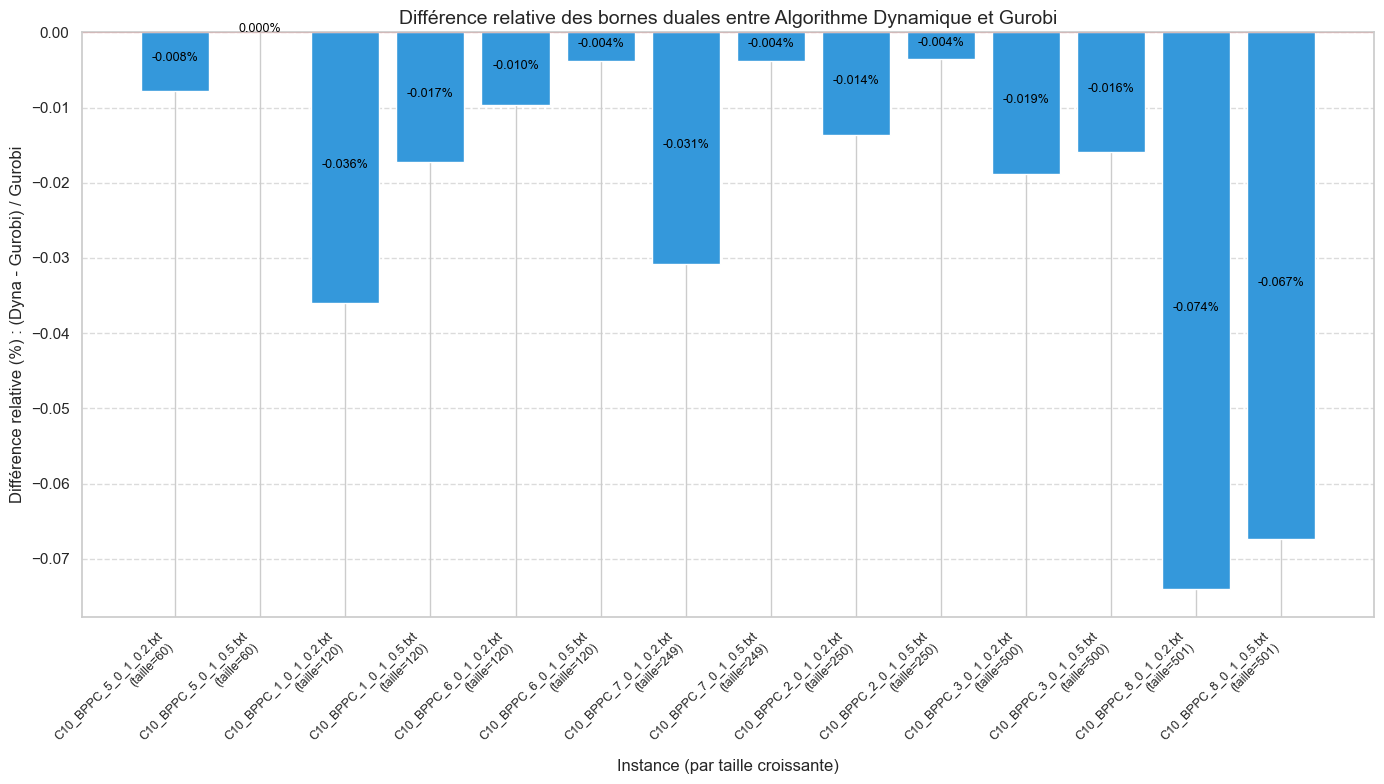
\includegraphics[width=1\textwidth]{diffDynaGuro.png}


	
	\subsection{Gestion des paramètres de la relaxation Lagrangienne}
	
	Comme évoqué précédemment, la volonté d'obtenir de bonne borne duale avec la relaxation Lagrangienne a nécessité l'implémentation d'un algorithme de sous-gradients pour optimiser au mieux la mise à jour du vecteur de pénalités Lagrangienne. Afin de permettre à notre algorithme de converger vers une bonne borne duale et de comprendre quels impact peuvent avoir la variation des paramètres ($\alpha$ et $M$), nous avons exécuté l'algorithme avec différents $\alpha \in \{ 0.1 x : x \in \{8,\dots,19\}\}$ et $M \in \{100 y : y \in \{1,\dots,5\}\}$. \\
	Le tableau suivant contient donc les principales informations (temps, alpha et M) associées à la meilleure borne duale trouvée pour chaque instance. 
	
	
	\begin{table}[htbp]
	\centering
	\label{tab:resultats_dyna}
	\begin{tabular}{lrrrrrr}
		\hline
		\textbf{Instance} & \textbf{Borne Duale} & \textbf{Borne Primale} & \textbf{Alpha} & \textbf{M} & \textbf{Temps (s)} & \textbf{Taille} \\
		\hline
		C10\_BPPC\_1\_0\_1\_0.2.txt & 1\,888.50 & 0.0 & 1.2 & 300 & 18.046 & 120 \\
		C10\_BPPC\_1\_0\_1\_0.5.txt & 1\,860.84 & 1\,850.0 & 1.1 & 200 & 12.808 & 120 \\
		C10\_BPPC\_2\_0\_1\_0.2.txt & 1\,980.89 & 1\,970.0 & 1.7 & 200 & 30.846 & 250 \\
		C10\_BPPC\_2\_0\_1\_0.5.txt & 1\,953.68 & 0.0 & 0.8 & 100 & 22.818 & 250 \\
		C10\_BPPC\_3\_0\_1\_0.2.txt & 2\,077.42 & 2\,070.0 & 1.8 & 200 & 53.776 & 500 \\
		C10\_BPPC\_3\_0\_1\_0.5.txt & 2\,066.24 & 2\,060.0 & 1.5 & 500 & 84.465 & 500 \\
		C10\_BPPC\_5\_0\_1\_0.2.txt & 10\,318.10 & 10\,310.0 & 1.5 & 500 & 66.784 & 60 \\
		C10\_BPPC\_5\_0\_1\_0.5.txt & 7\,543.00 & 7\,543.0 & 0.8 & 100 & 3.498 & 60 \\
		C10\_BPPC\_6\_0\_1\_0.2.txt & 10\,375.20 & 0.0 & 0.8 & 500 & 234.035 & 120 \\
		C10\_BPPC\_6\_0\_1\_0.5.txt & 10\,352.40 & 10\,350.0 & 0.9 & 400 & 122.050 & 120 \\
		C10\_BPPC\_7\_0\_1\_0.2.txt & 10\,390.00 & 0.0 & 0.8 & 100 & 22.322 & 249 \\
		C10\_BPPC\_7\_0\_1\_0.5.txt & 10\,390.00 & 0.0 & 0.8 & 100 & 23.199 & 249 \\
		C10\_BPPC\_8\_0\_1\_0.2.txt & 10\,390.00 & 10\,390.0 & 0.8 & 100 & 47.562 & 501 \\
		C10\_BPPC\_8\_0\_1\_0.5.txt & 10\,390.00 & 0.0 & 0.8 & 100 & 50.161 & 501 \\
		toy\_instance.txt & 17.04 & 17.0 & 0.8 & 100 & 0.009 & 7 \\
		\hline
	\end{tabular}
	\caption{Résultats de l'algorithme dynamique pour les différentes instances}
\end{table}
	
	
	Tout d'abord, nous observons  que pour certaines instances, l'obtention d'une bonne borne duale n'implique pas nécessairement une borne primale de bonne qualité. Etant donné que nous avons initialisé la borne primale à 0, nous constatons même que l'algorithme n'est jamais passé par une solution réalisable améliorante. Dans de rares cas, une solution optimale a pu être trouvée (l.8, l.13 et l.15).  \\
	Ensuite, nous observons un répartition des coefficients $\alpha$ très proche de 1, avec la majeur partie valant $0.8$. C'est ce que retranscrit le graphique suivant  : \\
	
	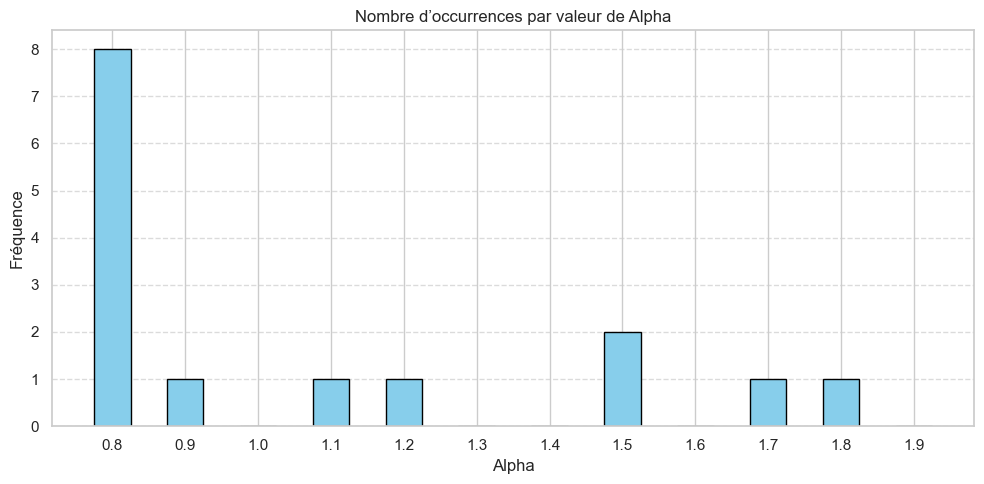
\includegraphics[width=0.9\textwidth]{bestAlpha.png}
	
Ainsi, dans plus de la moitié des cas, c'est pour $\alpha = 0.8$ que nous convergons le plus rapidement/efficacement vers une borne duale de qualité.  \\




Il était intéressant de comprendre quel impact le choix du nombre d'itérations maximum sans amélioration (de la borne duale) aurait sur une borne duale de bonne qualité. En éxécutant l'algorithme pour chaque instance avec $M  \in \{100,\dots,500\}$, nous avons conservé, pour chaque instance, la configuration ayant mené à la meilleure borne duale. Nous en déduisons que pour notre jeu de données, c'est le nombre le plus raisonnable d'itérations qui l'emporte, avec 100 répétitions maximum sans améliorations. Nous constatons également une représentation moyenne de $M = 500$, ce qui suggère que certaines instances ont besoin d'un plus grand nombre d'itérations pour converger vers une borne duale efficace. 

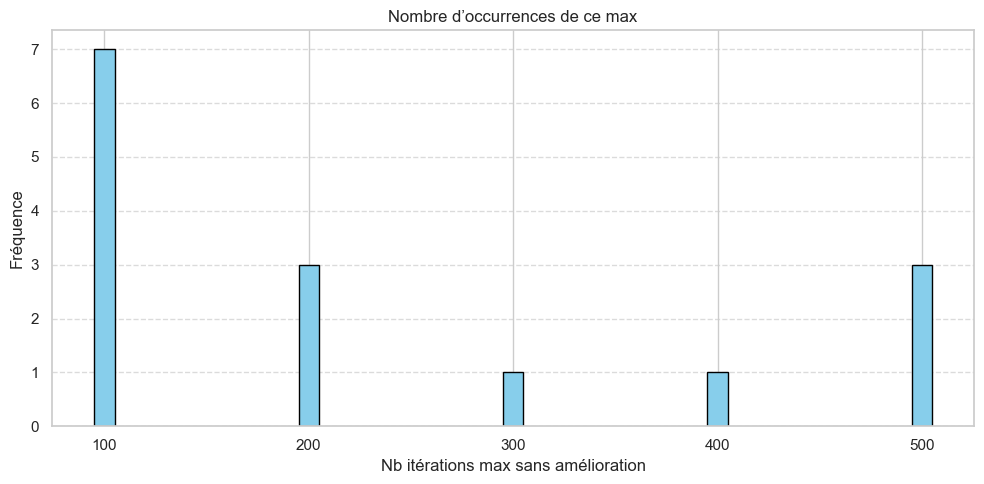
\includegraphics[width=0.9\textwidth]{bestM.png}



\end{document}